\documentclass{standalone}
\usepackage[utf8]{inputenc}
\usepackage[T1]{fontenc}
\usepackage{tikz}
\usetikzlibrary{positioning,fit,arrows.meta,shapes,calc}

\begin{document}

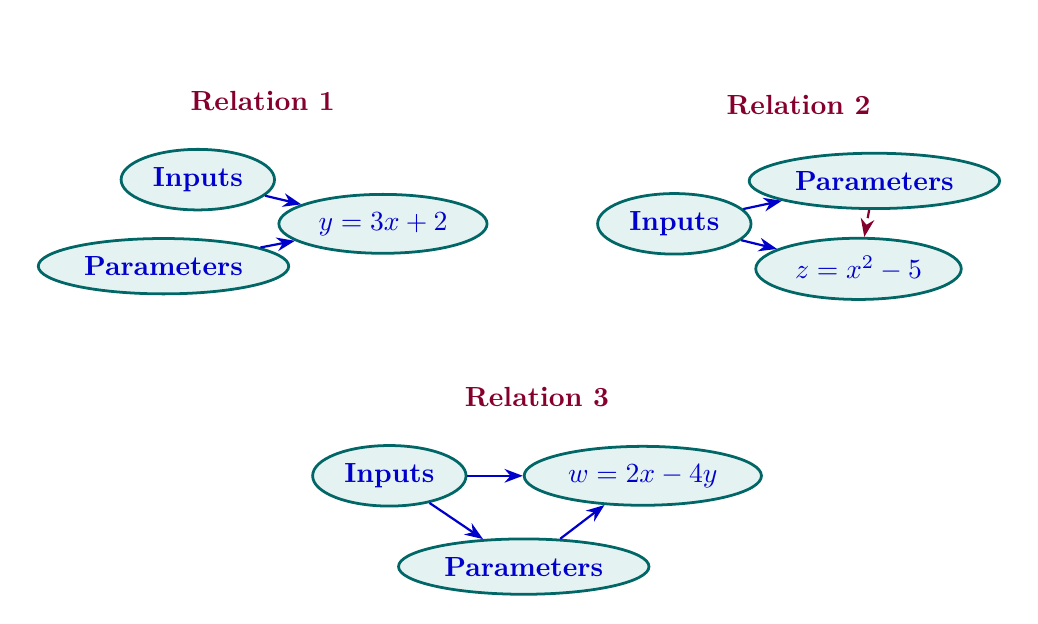
\begin{tikzpicture}[
  auto,
  >=Stealth,
  node distance = 0.0ex and 2em,
  rel/.style = {->, thick, color=blue!80!black},
  mathnode/.style = {
    ellipse,
    draw = teal!80!black,
    fill = teal!10,
    line width = 1pt,
    minimum width = 5em,
    minimum height = 2em,
    font = \bfseries\color{blue!80!black},
    align = center},
  labelnode/.style = {
    font = \bfseries\color{purple!70!black}
  }
  ]

% Synonyms and context update
\def\inputs{Inputs}
\def\outputs{Outputs}
\def\parameters{Parameters}
\def\mathnet{Mathematical Relation}

% First relationship cluster (left)
\begin{scope}
  \node[mathnode] (n1out) {$y=3x+2$};
  \node[mathnode, above left = of n1out] (n1in) {\inputs};
  \node[mathnode, below left = of n1out] (n1param) {\parameters};
  \path[rel] (n1in) edge (n1out);
  \path[rel] (n1param) edge (n1out);
  \node[fit = (n1in)(n1param)(n1out), above, yshift = 1em, labelnode] (fitA) {Relation 1};
\end{scope}

% Second relationship cluster (middle-right)
\begin{scope}[xshift = 3.7cm]
  \node[mathnode] (n2in) {\inputs};
  \node[mathnode, below right = of n2in] (n2out) {$z=x^2-5$};
  \node[mathnode, above right = of n2in] (n2param) {\parameters};
  \path[rel] (n2in) edge (n2out);
  \path[rel] (n2in) edge (n2param);
  \path[rel, dashed, color=purple!70!black] (n2param) edge (n2out);
  \node[fit = (n2in)(n2param)(n2out), above, yshift = 1em, labelnode] (fitB) {Relation 2};
\end{scope}

% Third relationship cluster (lower-right)
\begin{scope}[xshift = 3.3cm, yshift = -3.2cm]
  \node[mathnode] (n3out) {$w=2x-4y$};
  \node[mathnode, left = of n3out] (n3in) {\inputs};
  \node[mathnode, below left = 1.75em and -2em of n3out] (n3param) {\parameters};
  \path[rel] (n3in) edge (n3out);
  \path[rel] (n3param) edge (n3out);
  \path[rel] (n3in) edge (n3param);
  \node[fit = (n3in)(n3param)(n3out), above, yshift = 1em, labelnode] (fitC) {Relation 3};
\end{scope}

\end{tikzpicture}

\end{document}